%%
% The BIThesis Template for Bachelor Graduation Thesis
%
% 北京理工大学毕业设计(论文)第一章节 —— 使用 XeLaTeX 编译
%
% Copyright 2020-2022 BITNP
%
% This work may be distributed and/or modified under the
% conditions of the LaTeX Project Public License, either version 1.3
% of this license or (at your option) any later version.
% The latest version of this license is in
%   http://www.latex-project.org/lppl.txt
% and version 1.3 or later is part of all distributions of LaTeX
% version 2005/12/01 or later.
%
% This work has the LPPL maintenance status `maintained'.
%
% The Current Maintainer of this work is Feng Kaiyu.
%
% 第一章节

\chapter{绪论}

\section{研究背景}
三维场景地图的重建对三维计算机视觉、机器人学等领域有着重大意义,《“十四五”机器人产业发展规划》中指出,“机器人+”应用行动应该在汽车领域着力开发和推广。近年来, 国内外涌现了一大批优秀的自动驾驶企业,希望通过自动驾驶算法,在保证驾驶安全的前提下,逐步用计算机算法代替驾驶员来进行决策。然而,自动驾驶算法的落地过程并不是一帆风顺的,随着越来越多自动驾驶车辆由于算法缺陷导致的交通事故的出现,自动驾驶算法安全性愈发得到科研界、产业界的关注。为了不断提高自动驾驶算法安全性,研究者致力于实现从真实(Real)到仿真(Sim),再到真实的数据闭环,这一过程被称为Real2Sim2Real:
\begin{enumerate}
    \item \textbf{Real2Sim:} 从真实感知数据中进行三维重建,并建立仿真化环境,在仿真场景中不断迭代自动驾驶算法;
    \item \textbf{Sim2Real:}再将迭代后的算法重新部署到真实自动驾驶车辆中,而真实车辆运行过程中采集到的新数据可以被增补到仿真环境中,建立更富有真实感的仿真驾驶环境。
\end{enumerate}

而为了实现这一目的,则需要保证从Real2Sim得到的仿真三维重建场景可以做到与真实观测结果相匹配,否则从仿真器中迭代训练的自动驾驶算法很容易受到领域偏差的影响,从而在真实道路环境中产生安全隐患。

因此,本文着力于解决Real2Sim2Real的第一环,即Real2Sim的场景地图三维重建。本文发现在现存的视觉三维重建方法通常存在一系列问题。
由于自动驾驶算法通常需要多元传感信息的输入(如RGB图片、LiDAR等深度感知信息、GPS位置信息等),为了构建具有真实感的自动驾驶仿真器,需要在重建的仿真三维地图中,为自动驾驶算法Agent提供真实感的图片渲染、精确的深度信息和准确的位置信息。
因此对于一个应用于仿真场景搭建的三维重建方法,最受关注的几个性能指标包括渲染的RGB图片是否真实,以及其对地图中物体的几何结构表示的准确性。

为了真正实现从实际道路驾驶数据中重建一个精准的三维世界, 本课题中将解决以下几个重要的科研问题:
\begin{enumerate}
    \item \textbf{混合隐式场景表示学习}:现有三维重建方法大多通过显式建模场景中的几何单元(如“点”,“网格”等)实现对三维物理世界的感知,然而这类方法通常无法满足Real2Sim自动驾驶仿真器对于渲染、几何的共同要求。本文将结合近年来广受关注的隐式场景表示,探索“在理想情况下,通过多元传感器信息进行三维重建”这一问题,也即探索三维场景地图表征的极限能力。

    现有三维重建方法中使用传统显式的点云、栅格地图,只能根据传感器分辨率在有限分辨率对场景进行描述,对于存储的开销较大。近年来,基于神经网络的隐式地图得到了显著的发展,这类方法通过拟合一个隐式函数来对环境的关键物理量进行表征,从而对场景进行无限分辨率的表达。典型的隐式场有神经辐射场、神经有符号距离场等。

    然而现有传统方法或单一隐式场方法不能同时建模较好的场景外观和精确的几何,从而限制了其在下游应用场景上的应用。如果使用混合的隐式表征(即混合隐式场),能够同时渲染逼真图片并且对于环境的几何形状有较为准确的表达,将会对下游重定位任务的执行、自动驾驶技术的提升等有巨大的帮助。
    
    \begin{figure}[t]
        \centering
        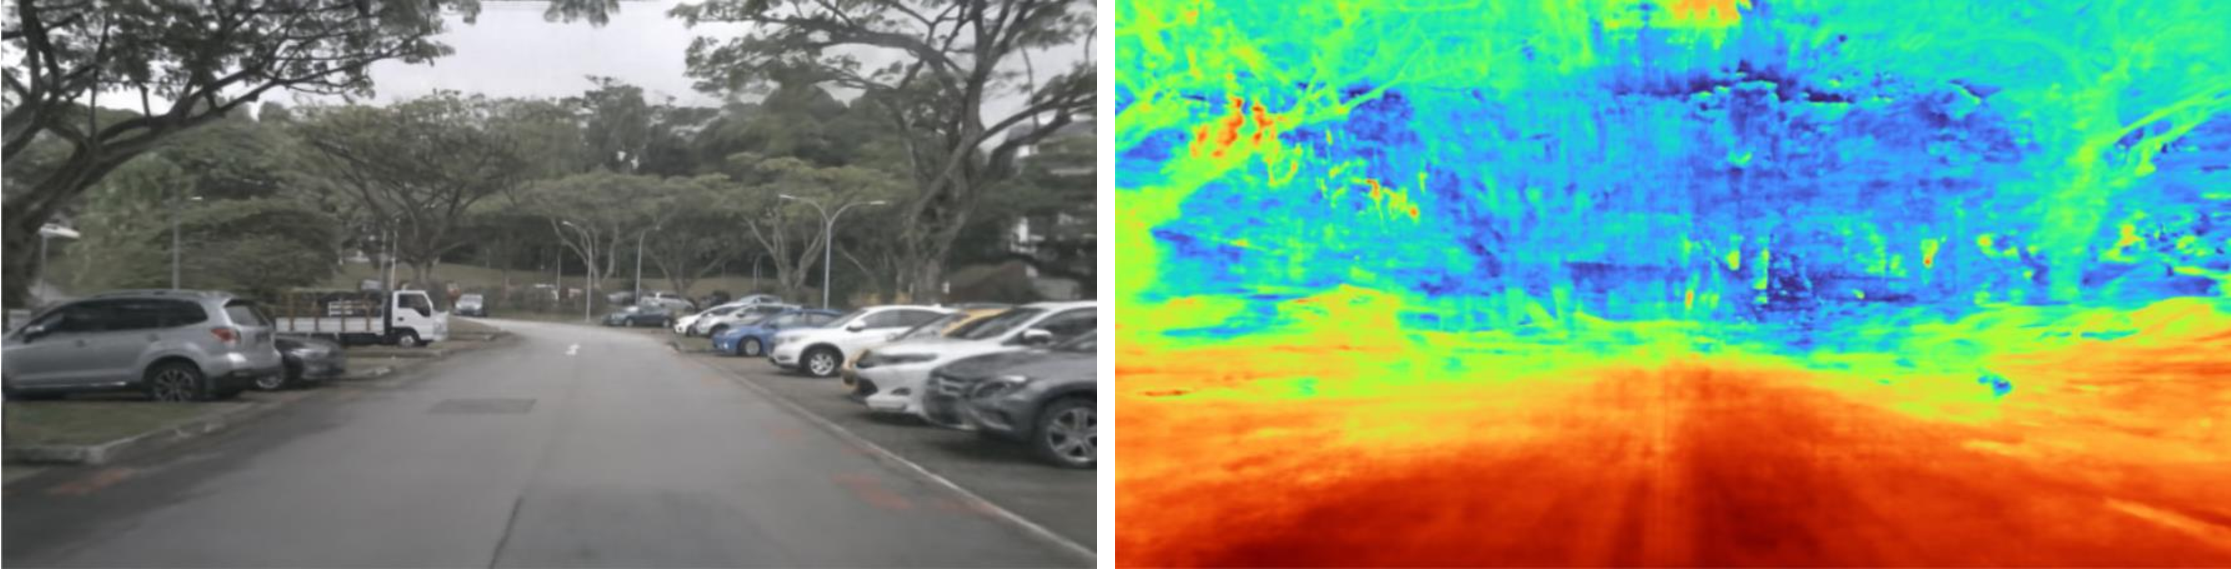
\includegraphics[width=0.9\textwidth]{undergraduate-thesis/images/RGB-D.pdf}
        \caption{左图为神经辐射场渲染的RGB图片,右图为同样位姿下渲染的深度图。可以看到辐射场对于场景外观信息建模能力较强, 但对于场景几何的学习效果较差。}
        \label{fig:rgb-d}
    \end{figure}
    
    % 除此以外,由于神经辐射场中仅用“辐射”代替物理光照模型中光的全部传播规律,因此不能用于灵活地改变环境光照
    现有混合隐式场方法尝试将距离函数映射为辐射场中用于体积积分的体密度\cite{wang_neus_2021, azinovic_neural_2022}。本文发现目前的混合隐式表征中存在诸多潜在的问题:
    \begin{itemize}
        \item 目前方法中,通常使用一个函数映射将距离值转换为体密度,本文观察到现有转换方法中存在多视角误差,将会对几何表示学习产生较大影响。
        \item 同时优化多种隐式表达本质上是一个多目标优化问题,如果不对训练过程进行约束,将会显著影响每个隐式函数的优化结果。
        \item 现有方法存在训练慢、模型大、无法泛化到大场景等问题。
    \end{itemize}
    
    如图\ref{fig:rgb-d}可见,仅从RGB图片的单一传感器输入训练神经辐射场获得的场景深度图与真实值存在较大误差。使用深度损失函数等方式融入深度感知数据,然而由于这些方法的隐式场景表达本身存在多视角误差,深度信息的引入反而会影响优化问题的进行。

    \item \textbf{面向真实自动驾驶数据的多元传感信息三维重建}:在上一个问题中,本文试图在理想状态下重建仿真场景地图,然而,要完成从真实到仿真,再从仿真到真实的数据闭环,必然要进行长时间的数据迭代,在这之中,必然会遇到退化的数据,那么如何在退化输入的情况下使得重建场景尽可能接近理想状态下的地图建模结果至关重要。在本文中,本文聚焦在真实自动驾驶数据中的两个重要问题:
    \begin{itemize}
        \item 在车端传感器框架下,通常会遇到传感器采样时间不不对齐的情况,如何在不添置昂贵的硬件设备的前提下从软件层面实现在线对齐则是一个亟待解决的问题。

        虽然现有方法可以分别在不同模态的传感信息上进行自动标定,但是他们均没有利用多元传感信息之间的共同轨迹先验信息,从而在精度上不足以支撑高保真的地图重建。
        
        \item 在真实道路环境中,可能会遇到各种不同的天气,其中以雾天为代表的散射现象对自动驾驶数据精度影响尤其显著,因为散射介质不仅影响了RGB相机的能见度,同时因为悬浮粒子对于激光的反射,会使得从激光雷达获取的深度信息不再可信。

        目前的视觉图像去雾方法虽然可以在一定程度上将带雾图片进行一定程度上的还原,但是现有方法通常局限在单视角的去雾上,从而无法利用多视角一致性信息。将一系列带雾图片输入到此类方法时,虽然处理后的每张图片看起来都是经过了去雾处理,但是原本存在于图片序列中的多视角一致性却会被破坏,从而给多视角三维重建算法带来更多挑战。
    \end{itemize}

    \item \textbf{真实动态场景仿真环境建模}:现有三维重建方法通常假设场景是恒久不变的静态场景,然而在真实道路环境中,行人、其他行驶车辆的出现显然打破了这一前提,从而给三维场景重建任务带来了巨大的挑战。虽然可以简单的通过语义模型将行人、车辆忽略,而仅仅重建静态的背景部分,然而通过这样方法获得的仿真三维场景由于动态的缺失也显然不能应用于Real2Sim2Real的数据闭环。因此如何建模场景中的动态物体也是一个重要的研究问题。
\end{enumerate}

\section{国内外研究现状}

神经辐射场(Neural Radiance Fields, NeRF)\cite{mildenhall_nerf_2020}最早被用于从已观测到的视角图片中学习场景信息,并渲染新视角下的图片,这类方法可以渲染高逼真的RGB图片。神经辐射场建立在一个简化的物理光照模型上:任意三维空间中的点均会向外散射不同颜色的光,从不同视角观察空间中的同一点的颜色可能不同,且每个点都会对其他方向传播过来的光线具有阻碍传播的作用。对三维点$P_i (x,y,z)$和观察角度$V(\theta,\phi)$,点$P_i$在角度V下观察到的颜色可以被一个五维连续隐式函数$f_{NeRF}:(x,y,z,\theta,\phi)\to (c_i,\sigma_i),c_i\in[0,255]^3,\sigma_i\in \mathbb{R}$ 建模,其中$c_i$为$P_i$散射出的RGB颜色值,而$\sigma_i$为该点的体密度。通过加权累积一条光线上所穿过点的辐射值,可以达到照片级的渲染,并且由于渲染过程的天然可微性,可以用渲染图片和观察到的图片之间的误差更新隐式函数$f_{NeRF}$。虽然神经辐射场可以精准地学习场景的视觉特征,然而仅从图片渲染误差中学习到的场景几何是缺乏约束的。因此,以神经辐射场为代表的方法在场景几何学习的深度估计等任务的精度要求上(如RMSE等指标)上的效果不足以支持“真实$\rightarrow$仿真$\rightarrow$真实”的任务要求,即将从视觉感知获得的几何表示应用于真实场景机器人实践应用(Real2Sim2Real)等更广泛的机器人应用。

在最初的神经辐射场中,研究者使用多层感知机(Multi-layer Perceptrons, MLP)来建模隐函数$f_{NeRF}$,在MonoSDF\cite{yu_monosdf_2022}, InstantNGP\cite{muller_instant_2022}等后续工作中提出使用MLP来建模该函数关系存在训练/渲染时间过长、建模能力差和遗忘等问题,并提出使用三维空间网格代替感知机学习隐函数表征。但使用三维网格建模场景信息存在模型体积大,无法泛化到大场景的问题,因此后续工作\cite{chen_tensorf_2022, fridovich-keil_k-planes_2023, cao_hexplane_2023, reiser_merf_2023}提出使用张量分解\cite{kolda_tensor_2009}的思想将三维张量分解为多个二维矩阵,从而将场景模型的空间复杂度从$\mathcal O (L^3)$降为$\mathcal O (L^2)$。本文总结现有隐式场表示的方法如下:
\begin{itemize}
    \item \textbf{多层感知机}:使用一个带残差的多层感知机分别学习混合隐式场表征。在查询时直接将空间点信息输入网络,直接预测隐函数值。如图\ref{fig:scene-representation} (a)所示。
    \item \textbf{空间体素网格}:使用一个空间体素网格存储空间中不同区域的隐式场真值,在推理时使用三线性插值计算任意给定三维空间中点的隐式函数值。如图\ref{fig:scene-representation} (b)所示。
    \item \textbf{多分辨率体素特征网格}:将三维空间按照不同分辨率分别建立空间体素网格,在网格中存储空间几何和外观的特征,并用三线性插值和一个浅层的解码器多层感知机推理隐函数值。
    \item \textbf{二维网格}:与空间体素网格相似,该类方法将隐式场表示为多个二维矩阵,在查询任意空间点的隐函数值时将该点投影到各个二维矩阵平面中,使用双线性插值得出投影点特征,将所有二维矩阵投影点的特征进行重新整合,得到最终查询点特征。如图\ref{fig:scene-representation} (c)所示。
    \item \textbf{混合表征}:同时多种相同或不同形式的隐式场表示方法。
\end{itemize}

\begin{figure}[t]
    \centering
    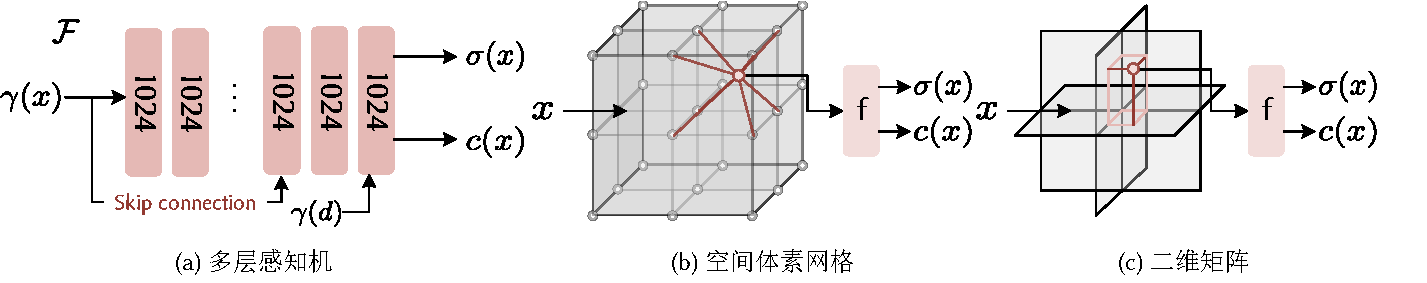
\includegraphics[width=\textwidth]{undergraduate-thesis/images/Scene Representations.pdf}
    \caption{场景表征示意图}
    \label{fig:scene-representation}
\end{figure}

相比神经辐射场主要通过图片中的特征学习场景的视觉信息,有符号距离场(Signed Distance Fields, SDF)可以用来表达更精确的场景几何信息。在有符号距离场 $f_{SDF}:(x,y,z)→d_i$中,任意空间点$P_i$被映射到其距离最近的表面的有符号距离$d_i\in \mathbb{R}$。通过从RGB图片中抽取多视角几何对应关系,或从深度图像中获取场景几何的直接观测结果,现有方法可以通过视觉感知输入重建较为准确的场景模型。然而这类方法通常无法得到逼真的RGB渲染图片。

\section{本课题主要工作及主要创新点}

近年来,混合隐式表达逐渐被研究者所关注,NeuS\cite{wang_neus_2021}方法首先提出了将辐射场和距离场相结合的范式,即建立距离到体密度的映射关系,然而该方法仅考虑了单视角下的无偏和遮挡,而没用考虑多视角的一致性,此外,该方法仅从RGB图片中学习场景表示,而不能利用深度图片的信息。NeuralRGB-D\cite{azinovic_neural_2022}方法在NeuS的基础上,使用了深度图来作为额外的场景感知输入。这些现有方法简单地将辐射场和距离场表达相结合,会使得整个优化任务的难度大大提升,从而显著地影响模型的整体性能。 因此,如何将不同的隐式函数有效地结合便成为当下隐式场研究的一个核心问题。为此,本课题首先考虑在场景的密度信息和梯度信息之间建立桥梁,保证混合隐式场在多视角下的空间一致性,实现距离场和辐射场的同时协同优化,以期解决隐式场的优化问题。除此以外,目前方法在表达大场景上存在严重的泛化问题,即训练速度极慢、模型大、效果差等。在本课题中,本文使用多元传感输入(包括RGB相机、激光雷达或深度相机等),将不同模态下的传感数据进行融合,来优化混合隐式场表征。所得的混合隐式场应能被用于真实感的图像渲染、高保真深度预测和三维重建等应用场景。


\begin{figure}[t]
    \centering
    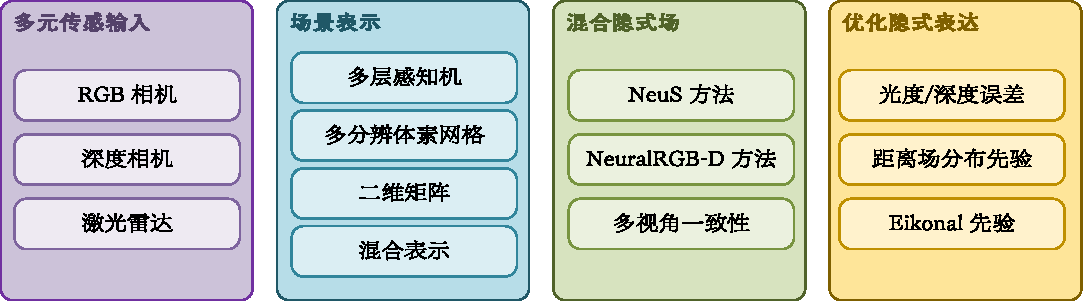
\includegraphics[width=\textwidth]{undergraduate-thesis/images/method.pdf}
    \caption{本课题中采用的技术路线}
    \label{fig:method}
\end{figure}

在此基础之上,为了解决真实自动驾驶场景中所遇到的退化输入数据,本文分别在多元传感器时间同步和雾天受散射效应影响较大两个问题上提出解决方案。为了实现对室外场景中的动态物体进行主动建模,本文通过将场景分解成场景图网络,在建模动态物体的基础上实现了对车辆行驶轨迹和外观进行编辑。

综上,本文的主要创新点和技术贡献如下:
\begin{itemize}
    \item 本文结合现有方法中不同的隐式场种类、隐式场表达,建立了基于多元传感信息输入的混合距离-辐射场,可以在场景外观颜色渲染和场景几何建模等任务超过现有方法。
    \item 从异步 RGBD 序列训练城市规模的神经辐射场,解决了现实应用中遇到的实际问题。本文在这个问题中确定了一个重要的特定领域先验:RGB-D 帧是从相同的基础轨迹中采样的。本文先将其实例化为一个新颖的时间-姿势函数,并开发一个级联隐式表示网络。
    \item 本文首次提出从带雾图像中学习神经隐式场,通过对采样点的权重进行重新配置,使得可以准确将悬浮粒子和场景的结构解耦,利用带雾图像中的隐式深度信息作为RGB图片的增补,从而实现高质量的隐式场景表示学习,并允许灵活的散射效应控制。
    \item 本文从RGB-D真实数据中学习混合隐式场景图,实现了对动态场景的理解和编辑。通过将上述技术贡献进行整合,可以实现从真实多元传感的自动驾驶数据中构建隐式自动驾驶仿真环境,从而实质性推动自动驾驶Real2Sim2Real的技术发展。
    \item 本文在公开数据集和在各种退化条件下在仿真、真实场景中采集数据上进行详尽的对比实验,验证了本课题所提出方法显著优于现有方法。
\end{itemize}

\section{本文章节安排}
本文分成六个章节,第一章(本章节)阐述本文的研究背景、意义,分析在Real2Sim2Real数据闭环的需求下为了实现Real2Sim仿真场景重建所需要解决的困难,介绍与混合隐式表达相关国内外相关工作,并最后介绍本文的主要研究工作和创新点。

第二章介绍了混合隐式场景表示这一新兴领域的相关理论和主流方法。该章首先介绍神经隐式场景表示的概念,以及场景表示模型从多层感知机逐渐演变的过程, 接着介绍用于真实感渲染的神经隐式场理论和技巧,但这一部分均只局限于单一的隐式表征,在后半部分将转而介绍同时用于精准建模场景外观和几何的混合隐式场景表示。

第三章中介绍了本文所提出的神经混合隐式场的理论框架,解决在理想情况多元传感数据输入情况下高精度建模的问题,并为后续章节提供基础。这一章中首先分析现有距离-辐射混合隐式表达中由于距离到体密度映射过程的缺陷所带来的两种误差,由这两个误差引出本文所提出的基于全方向距离场的混合隐式表达。 在此基础上,本文进而引入抗锯齿技术,以进一步提升渲染画面质量。然而这一方法只能解决理想状态下,即多元传感器均在时间上同步,且在光照、天气较为理想的情况时的高精度建模问题。

第四章介绍了本文为了实现在真实自动驾驶数据中重建高精度地图表征的一系列方法。首先,本文分析了室外数据中广泛存在但没有被解决的传感器同步问题,通过引入隐式轨迹函数(TPF),并在建图阶段持续优化,本文可以在多传感器时间异步的退化条件下获得与理想情况下相匹配的建图结果。在第四章的后半部分,本文讨论了在带雾、下雨天气等受空间散射效应影响严重的情况下,进行地图重建的问题。在这类天气下,深度传感器无法产生可信的数据,而RGB相机也会受到光线散射的影响,从而显著降低能见度。 本文通过分析散射光照模型,通过采样点重赋权、协方差损失等方法,实现与正常天气几乎一样的建图结果,并能渲染高清无雾图片。

第五章介绍了基于本文提出的混合神经隐式场构建的动态场景图。本文在前四章所介绍的方法均只能处理静态场景的建模,而为了实现Real2Sim仿真器,就需要对其中的动态物体进行单独建模,因此在这一章中介绍了使用场景图分解的方法重建动态场景的技术路线,其中被分解的每个子模型均为前文提到的混合隐式场景表征模型。在最后,该章介绍了使用训练好的场景图模型可以实现Real2Sim仿真器所需要的场景编辑能力。

第六章介绍为了验证本文中提出方法所进行的一系列分析实验和结果。在这一章中首先列出实验所使用的数据集,其中包含公开数据集和本文在真实场景下不同步和带雾两种退化场景下所构建的数据集,并介绍模型评估指标。接下来介绍本文所进行的一系列详尽的实验以验证方法有效性,除了与基线模型的对比,该章还介绍了模型中每个组件的消融实验。

本文的最后总结了全文研究工作,并展望了未来可能的可扩展研究方向。